\documentclass{standalone}
\usepackage{tikz}
\usetikzlibrary{patterns, positioning}

\begin{document}
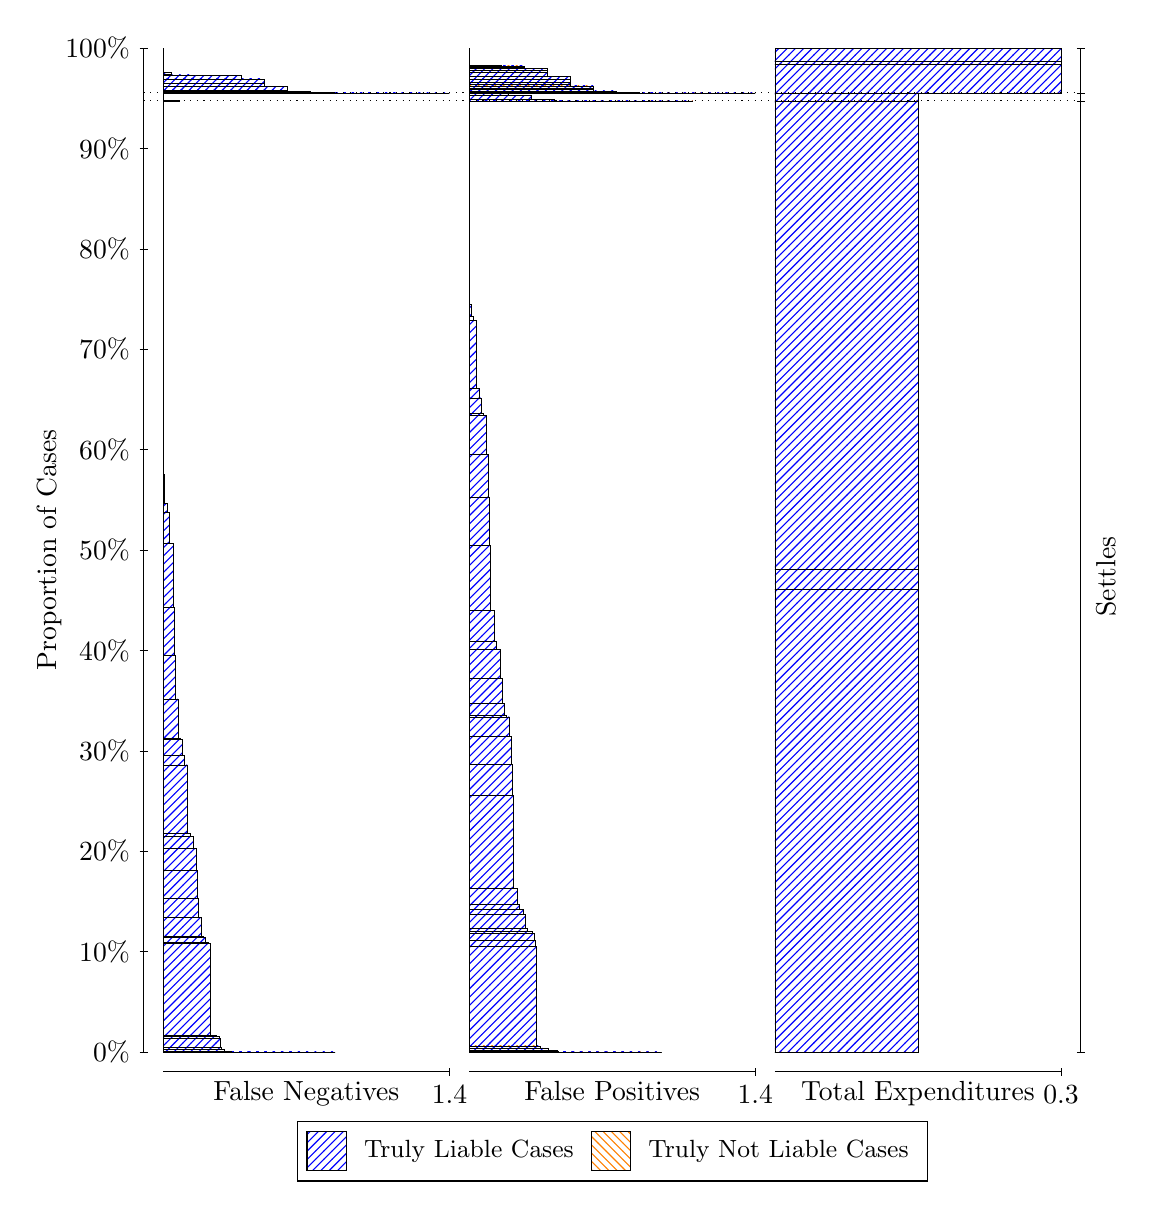
\begin{tikzpicture}
\draw[black, very thin] (1.5,1.75) -- (1.5,14.5);
\node[rotate=90, anchor=center] at (0.3, 8.125) {Proportion of Cases};
\draw[black, very thin] (1.45,1.75) -- (1.55,1.75);
\node[anchor=east] at (1.45, 1.75) {0\%};
\draw[black, very thin] (1.45,3.025) -- (1.55,3.025);
\node[anchor=east] at (1.45, 3.025) {10\%};
\draw[black, very thin] (1.45,4.3) -- (1.55,4.3);
\node[anchor=east] at (1.45, 4.3) {20\%};
\draw[black, very thin] (1.45,5.575) -- (1.55,5.575);
\node[anchor=east] at (1.45, 5.575) {30\%};
\draw[black, very thin] (1.45,6.85) -- (1.55,6.85);
\node[anchor=east] at (1.45, 6.85) {40\%};
\draw[black, very thin] (1.45,8.125) -- (1.55,8.125);
\node[anchor=east] at (1.45, 8.125) {50\%};
\draw[black, very thin] (1.45,9.4) -- (1.55,9.4);
\node[anchor=east] at (1.45, 9.4) {60\%};
\draw[black, very thin] (1.45,10.675) -- (1.55,10.675);
\node[anchor=east] at (1.45, 10.675) {70\%};
\draw[black, very thin] (1.45,11.95) -- (1.55,11.95);
\node[anchor=east] at (1.45, 11.95) {80\%};
\draw[black, very thin] (1.45,13.225) -- (1.55,13.225);
\node[anchor=east] at (1.45, 13.225) {90\%};
\draw[black, very thin] (1.45,14.5) -- (1.55,14.5);
\node[anchor=east] at (1.45, 14.5) {100\%};

\draw[black, very thin] (13.4,1.75) -- (13.4,14.5);
\draw[black, very thin] (13.35,1.75) -- (13.45,1.75);
\node[anchor=west] at (13.35, 1.75) {};
\draw[black, very thin] (13.35,13.828) -- (13.45,13.828);
\node[anchor=west] at (13.35, 13.828) {};
\draw[black, very thin] (13.35,13.931) -- (13.45,13.931);
\node[anchor=west] at (13.35, 13.931) {};
\draw[black, very thin] (13.35,14.5) -- (13.45,14.5);
\node[anchor=west] at (13.35, 14.5) {};

\draw[black, very thin, pattern color=blue, pattern=north east lines] (1.75,1.75) rectangle (3.93,1.75);
\draw[black, very thin, pattern color=blue, pattern=north east lines] (1.75,1.75) rectangle (3.6658,1.75);
\draw[black, very thin, pattern color=blue, pattern=north east lines] (1.75,1.75) rectangle (3.6364,1.75);
\draw[black, very thin, pattern color=blue, pattern=north east lines] (1.75,1.75) rectangle (3.4015,1.75);
\draw[black, very thin, pattern color=blue, pattern=north east lines] (1.75,1.75) rectangle (3.3722,1.75);
\draw[black, very thin, pattern color=blue, pattern=north east lines] (1.75,1.75) rectangle (3.3428,1.75);
\draw[black, very thin, pattern color=blue, pattern=north east lines] (1.75,1.75) rectangle (3.2694,1.75);
\draw[black, very thin, pattern color=blue, pattern=north east lines] (1.75,1.75) rectangle (3.1373,1.75);
\draw[black, very thin, pattern color=blue, pattern=north east lines] (1.75,1.75) rectangle (3.1079,1.75);
\draw[black, very thin, pattern color=blue, pattern=north east lines] (1.75,1.75) rectangle (3.0786,1.75);
\draw[black, very thin, pattern color=blue, pattern=north east lines] (1.75,1.75) rectangle (3.0492,1.75);
\draw[black, very thin, pattern color=blue, pattern=north east lines] (1.75,1.75) rectangle (3.0052,1.75);
\draw[black, very thin, pattern color=blue, pattern=north east lines] (1.75,1.75) rectangle (2.9758,1.75);
\draw[black, very thin, pattern color=blue, pattern=north east lines] (1.75,1.75) rectangle (2.873,1.7504);
\draw[black, very thin, pattern color=blue, pattern=north east lines] (1.75,1.7504) rectangle (2.8437,1.7504);
\draw[black, very thin, pattern color=blue, pattern=north east lines] (1.75,1.7504) rectangle (2.8143,1.751);
\draw[black, very thin, pattern color=blue, pattern=north east lines] (1.75,1.751) rectangle (2.7849,1.7515);
\draw[black, very thin, pattern color=blue, pattern=north east lines] (1.75,1.7515) rectangle (2.7556,1.752);
\draw[black, very thin, pattern color=blue, pattern=north east lines] (1.75,1.752) rectangle (2.7115,1.7523);
\draw[black, very thin, pattern color=blue, pattern=north east lines] (1.75,1.7523) rectangle (2.6822,1.7524);
\draw[black, very thin, pattern color=blue, pattern=north east lines] (1.75,1.7524) rectangle (2.6088,1.7528);
\draw[black, very thin, pattern color=blue, pattern=north east lines] (1.75,1.7528) rectangle (2.5794,1.761);
\draw[black, very thin, pattern color=blue, pattern=north east lines] (1.75,1.761) rectangle (2.5501,1.7613);
\draw[black, very thin, pattern color=blue, pattern=north east lines] (1.75,1.7613) rectangle (2.5207,1.7869);
\draw[black, very thin, pattern color=blue, pattern=north east lines] (1.75,1.7869) rectangle (2.4913,1.8127);
\draw[black, very thin, pattern color=blue, pattern=north east lines] (1.75,1.8127) rectangle (2.4767,1.9212);
\draw[black, very thin, pattern color=blue, pattern=north east lines] (1.75,1.9212) rectangle (2.462,1.9475);
\draw[black, very thin, pattern color=blue, pattern=north east lines] (1.75,1.9475) rectangle (2.4179,1.962);
\draw[black, very thin, pattern color=blue, pattern=north east lines] (1.75,1.962) rectangle (2.3886,1.9653);
\draw[black, very thin, pattern color=blue, pattern=north east lines] (1.75,1.9653) rectangle (2.3445,3.126);
\draw[black, very thin, pattern color=blue, pattern=north east lines] (1.75,3.126) rectangle (2.3152,3.1393);
\draw[black, very thin, pattern color=blue, pattern=north east lines] (1.75,3.1393) rectangle (2.2858,3.2096);
\draw[black, very thin, pattern color=blue, pattern=north east lines] (1.75,3.2096) rectangle (2.2565,3.2137);
\draw[black, very thin, pattern color=blue, pattern=north east lines] (1.75,3.2137) rectangle (2.2271,3.4545);
\draw[black, very thin, pattern color=blue, pattern=north east lines] (1.75,3.4545) rectangle (2.1977,3.7002);
\draw[black, very thin, pattern color=blue, pattern=north east lines] (1.75,3.7002) rectangle (2.1831,4.0591);
\draw[black, very thin, pattern color=blue, pattern=north east lines] (1.75,4.0591) rectangle (2.1684,4.3309);
\draw[black, very thin, pattern color=blue, pattern=north east lines] (1.75,4.3309) rectangle (2.1243,4.4906);
\draw[black, very thin, pattern color=blue, pattern=north east lines] (1.75,4.4906) rectangle (2.095,4.5325);
\draw[black, very thin, pattern color=blue, pattern=north east lines] (1.75,4.5325) rectangle (2.0509,5.3947);
\draw[black, very thin, pattern color=blue, pattern=north east lines] (1.75,5.3947) rectangle (2.0216,5.521);
\draw[black, very thin, pattern color=blue, pattern=north east lines] (1.75,5.521) rectangle (1.9922,5.7211);
\draw[black, very thin, pattern color=blue, pattern=north east lines] (1.75,5.7211) rectangle (1.9629,5.7381);
\draw[black, very thin, pattern color=blue, pattern=north east lines] (1.75,5.7381) rectangle (1.9335,6.2356);
\draw[black, very thin, pattern color=blue, pattern=north east lines] (1.75,6.2356) rectangle (1.9041,6.7864);
\draw[black, very thin, pattern color=blue, pattern=north east lines] (1.75,6.7864) rectangle (1.8895,7.3961);
\draw[black, very thin, pattern color=blue, pattern=north east lines] (1.75,7.3961) rectangle (1.8748,8.2162);
\draw[black, very thin, pattern color=blue, pattern=north east lines] (1.75,8.2162) rectangle (1.8307,8.6078);
\draw[black, very thin, pattern color=blue, pattern=north east lines] (1.75,8.6078) rectangle (1.8014,8.7136);
\draw[black, very thin, pattern color=blue, pattern=north east lines] (1.75,8.7136) rectangle (1.7573,9.083);
\draw[black, very thin, pattern color=orange, pattern=north west lines] (1.75,9.083) rectangle (1.75,9.083);
\draw[black, very thin, pattern color=blue, pattern=north east lines] (1.75,9.083) rectangle (1.75,13.828);
\draw[black, very thin, pattern color=blue, pattern=north east lines] (1.75,13.828) rectangle (1.9482,13.832);
\draw[black, very thin, pattern color=orange, pattern=north west lines] (1.75,13.832) rectangle (1.75,13.832);
\draw[black, very thin, pattern color=blue, pattern=north east lines] (1.75,13.832) rectangle (1.75,13.931);
\draw[black, very thin, pattern color=blue, pattern=north east lines] (1.75,13.931) rectangle (5.3833,13.931);
\draw[black, very thin, pattern color=blue, pattern=north east lines] (1.75,13.931) rectangle (5.0897,13.931);
\draw[black, very thin, pattern color=blue, pattern=north east lines] (1.75,13.931) rectangle (4.7961,13.931);
\draw[black, very thin, pattern color=blue, pattern=north east lines] (1.75,13.931) rectangle (4.5025,13.931);
\draw[black, very thin, pattern color=blue, pattern=north east lines] (1.75,13.931) rectangle (4.5025,13.931);
\draw[black, very thin, pattern color=blue, pattern=north east lines] (1.75,13.931) rectangle (4.2089,13.931);
\draw[black, very thin, pattern color=blue, pattern=north east lines] (1.75,13.931) rectangle (3.9153,13.934);
\draw[black, very thin, pattern color=blue, pattern=north east lines] (1.75,13.934) rectangle (3.6217,13.941);
\draw[black, very thin, pattern color=blue, pattern=north east lines] (1.75,13.941) rectangle (3.6217,13.954);
\draw[black, very thin, pattern color=blue, pattern=north east lines] (1.75,13.954) rectangle (3.3281,13.968);
\draw[black, very thin, pattern color=blue, pattern=north east lines] (1.75,13.968) rectangle (3.3281,14.015);
\draw[black, very thin, pattern color=blue, pattern=north east lines] (1.75,14.015) rectangle (3.3134,14.015);
\draw[black, very thin, pattern color=blue, pattern=north east lines] (1.75,14.015) rectangle (3.0345,14.048);
\draw[black, very thin, pattern color=blue, pattern=north east lines] (1.75,14.048) rectangle (3.0345,14.101);
\draw[black, very thin, pattern color=blue, pattern=north east lines] (1.75,14.101) rectangle (3.0345,14.107);
\draw[black, very thin, pattern color=blue, pattern=north east lines] (1.75,14.107) rectangle (3.0198,14.107);
\draw[black, very thin, pattern color=blue, pattern=north east lines] (1.75,14.107) rectangle (3.0198,14.107);
\draw[black, very thin, pattern color=blue, pattern=north east lines] (1.75,14.107) rectangle (2.7409,14.151);
\draw[black, very thin, pattern color=blue, pattern=north east lines] (1.75,14.151) rectangle (2.7262,14.151);
\draw[black, very thin, pattern color=blue, pattern=north east lines] (1.75,14.151) rectangle (2.4473,14.152);
\draw[black, very thin, pattern color=blue, pattern=north east lines] (1.75,14.152) rectangle (2.4473,14.155);
\draw[black, very thin, pattern color=blue, pattern=north east lines] (1.75,14.155) rectangle (2.4473,14.156);
\draw[black, very thin, pattern color=blue, pattern=north east lines] (1.75,14.156) rectangle (2.4326,14.156);
\draw[black, very thin, pattern color=blue, pattern=north east lines] (1.75,14.156) rectangle (2.4326,14.156);
\draw[black, very thin, pattern color=blue, pattern=north east lines] (1.75,14.156) rectangle (2.1537,14.156);
\draw[black, very thin, pattern color=blue, pattern=north east lines] (1.75,14.156) rectangle (2.1537,14.156);
\draw[black, very thin, pattern color=blue, pattern=north east lines] (1.75,14.156) rectangle (2.139,14.158);
\draw[black, very thin, pattern color=blue, pattern=north east lines] (1.75,14.158) rectangle (1.8601,14.158);
\draw[black, very thin, pattern color=blue, pattern=north east lines] (1.75,14.158) rectangle (1.8601,14.158);
\draw[black, very thin, pattern color=blue, pattern=north east lines] (1.75,14.158) rectangle (1.8454,14.161);
\draw[black, very thin, pattern color=blue, pattern=north east lines] (1.75,14.161) rectangle (1.8454,14.187);
\draw[black, very thin, pattern color=orange, pattern=north west lines] (1.75,14.187) rectangle (1.75,14.187);
\draw[black, very thin, pattern color=blue, pattern=north east lines] (1.75,14.187) rectangle (1.75,14.5);
\draw[black, very thin, pattern color=orange, pattern=north west lines] (5.6333,1.75) rectangle (8.0776,1.75);
\draw[black, very thin, pattern color=blue, pattern=north east lines] (5.6333,1.75) rectangle (8.0776,1.75);
\draw[black, very thin, pattern color=orange, pattern=north west lines] (5.6333,1.75) rectangle (7.9455,1.75);
\draw[black, very thin, pattern color=blue, pattern=north east lines] (5.6333,1.75) rectangle (7.9455,1.75);
\draw[black, very thin, pattern color=orange, pattern=north west lines] (5.6333,1.75) rectangle (7.8133,1.75);
\draw[black, very thin, pattern color=blue, pattern=north east lines] (5.6333,1.75) rectangle (7.8133,1.75);
\draw[black, very thin, pattern color=blue, pattern=north east lines] (5.6333,1.75) rectangle (7.784,1.75);
\draw[black, very thin, pattern color=blue, pattern=north east lines] (5.6333,1.75) rectangle (7.6519,1.75);
\draw[black, very thin, pattern color=orange, pattern=north west lines] (5.6333,1.75) rectangle (7.5491,1.75);
\draw[black, very thin, pattern color=blue, pattern=north east lines] (5.6333,1.75) rectangle (7.5491,1.75);
\draw[black, very thin, pattern color=blue, pattern=north east lines] (5.6333,1.75) rectangle (7.5197,1.75);
\draw[black, very thin, pattern color=blue, pattern=north east lines] (5.6333,1.75) rectangle (7.4904,1.75);
\draw[black, very thin, pattern color=orange, pattern=north west lines] (5.6333,1.75) rectangle (7.417,1.75);
\draw[black, very thin, pattern color=blue, pattern=north east lines] (5.6333,1.75) rectangle (7.417,1.75);
\draw[black, very thin, pattern color=blue, pattern=north east lines] (5.6333,1.75) rectangle (7.3582,1.75);
\draw[black, very thin, pattern color=orange, pattern=north west lines] (5.6333,1.75) rectangle (7.2848,1.75);
\draw[black, very thin, pattern color=blue, pattern=north east lines] (5.6333,1.75) rectangle (7.2848,1.75);
\draw[black, very thin, pattern color=blue, pattern=north east lines] (5.6333,1.75) rectangle (7.2555,1.75);
\draw[black, very thin, pattern color=blue, pattern=north east lines] (5.6333,1.75) rectangle (7.2261,1.75);
\draw[black, very thin, pattern color=blue, pattern=north east lines] (5.6333,1.75) rectangle (7.1968,1.75);
\draw[black, very thin, pattern color=orange, pattern=north west lines] (5.6333,1.75) rectangle (7.1527,1.75);
\draw[black, very thin, pattern color=blue, pattern=north east lines] (5.6333,1.75) rectangle (7.1527,1.75);
\draw[black, very thin, pattern color=blue, pattern=north east lines] (5.6333,1.75) rectangle (7.1234,1.75);
\draw[black, very thin, pattern color=blue, pattern=north east lines] (5.6333,1.75) rectangle (7.0646,1.75);
\draw[black, very thin, pattern color=orange, pattern=north west lines] (5.6333,1.75) rectangle (7.0206,1.75);
\draw[black, very thin, pattern color=blue, pattern=north east lines] (5.6333,1.75) rectangle (7.0206,1.75);
\draw[black, very thin, pattern color=blue, pattern=north east lines] (5.6333,1.75) rectangle (6.9912,1.75);
\draw[black, very thin, pattern color=blue, pattern=north east lines] (5.6333,1.75) rectangle (6.9619,1.7501);
\draw[black, very thin, pattern color=blue, pattern=north east lines] (5.6333,1.7501) rectangle (6.9325,1.7506);
\draw[black, very thin, pattern color=blue, pattern=north east lines] (5.6333,1.7506) rectangle (6.9032,1.7506);
\draw[black, very thin, pattern color=blue, pattern=north east lines] (5.6333,1.7506) rectangle (6.8591,1.7509);
\draw[black, very thin, pattern color=blue, pattern=north east lines] (5.6333,1.7509) rectangle (6.8298,1.7514);
\draw[black, very thin, pattern color=blue, pattern=north east lines] (5.6333,1.7514) rectangle (6.771,1.7548);
\draw[black, very thin, pattern color=orange, pattern=north west lines] (5.6333,1.7548) rectangle (6.7564,1.7548);
\draw[black, very thin, pattern color=blue, pattern=north east lines] (5.6333,1.7548) rectangle (6.7564,1.7662);
\draw[black, very thin, pattern color=blue, pattern=north east lines] (5.6333,1.7662) rectangle (6.727,1.7668);
\draw[black, very thin, pattern color=blue, pattern=north east lines] (5.6333,1.7668) rectangle (6.6976,1.767);
\draw[black, very thin, pattern color=blue, pattern=north east lines] (5.6333,1.767) rectangle (6.6683,1.7683);
\draw[black, very thin, pattern color=blue, pattern=north east lines] (5.6333,1.7683) rectangle (6.6389,1.7909);
\draw[black, very thin, pattern color=blue, pattern=north east lines] (5.6333,1.7909) rectangle (6.6096,1.7944);
\draw[black, very thin, pattern color=blue, pattern=north east lines] (5.6333,1.7944) rectangle (6.5655,1.8017);
\draw[black, very thin, pattern color=blue, pattern=north east lines] (5.6333,1.8017) rectangle (6.5362,1.8261);
\draw[black, very thin, pattern color=orange, pattern=north west lines] (5.6333,1.8261) rectangle (6.4921,1.8261);
\draw[black, very thin, pattern color=blue, pattern=north east lines] (5.6333,1.8261) rectangle (6.4921,3.0892);
\draw[black, very thin, pattern color=blue, pattern=north east lines] (5.6333,3.0892) rectangle (6.4774,3.1643);
\draw[black, very thin, pattern color=blue, pattern=north east lines] (5.6333,3.1643) rectangle (6.4628,3.2546);
\draw[black, very thin, pattern color=blue, pattern=north east lines] (5.6333,3.2546) rectangle (6.4334,3.2806);
\draw[black, very thin, pattern color=blue, pattern=north east lines] (5.6333,3.2806) rectangle (6.404,3.2837);
\draw[black, very thin, pattern color=blue, pattern=north east lines] (5.6333,3.2837) rectangle (6.3747,3.3152);
\draw[black, very thin, pattern color=blue, pattern=north east lines] (5.6333,3.3152) rectangle (6.3453,3.5);
\draw[black, very thin, pattern color=blue, pattern=north east lines] (5.6333,3.5) rectangle (6.316,3.5639);
\draw[black, very thin, pattern color=blue, pattern=north east lines] (5.6333,3.5639) rectangle (6.2719,3.6197);
\draw[black, very thin, pattern color=blue, pattern=north east lines] (5.6333,3.6197) rectangle (6.2426,3.8339);
\draw[black, very thin, pattern color=blue, pattern=north east lines] (5.6333,3.8339) rectangle (6.1985,5.0098);
\draw[black, very thin, pattern color=blue, pattern=north east lines] (5.6333,5.0098) rectangle (6.1838,5.4035);
\draw[black, very thin, pattern color=blue, pattern=north east lines] (5.6333,5.4035) rectangle (6.1692,5.7653);
\draw[black, very thin, pattern color=blue, pattern=north east lines] (5.6333,5.7653) rectangle (6.1398,6.0062);
\draw[black, very thin, pattern color=blue, pattern=north east lines] (5.6333,6.0062) rectangle (6.1104,6.0217);
\draw[black, very thin, pattern color=blue, pattern=north east lines] (5.6333,6.0217) rectangle (6.0811,6.1808);
\draw[black, very thin, pattern color=blue, pattern=north east lines] (5.6333,6.1808) rectangle (6.0517,6.4949);
\draw[black, very thin, pattern color=blue, pattern=north east lines] (5.6333,6.4949) rectangle (6.0224,6.8643);
\draw[black, very thin, pattern color=blue, pattern=north east lines] (5.6333,6.8643) rectangle (5.9783,6.9701);
\draw[black, very thin, pattern color=blue, pattern=north east lines] (5.6333,6.9701) rectangle (5.949,7.3617);
\draw[black, very thin, pattern color=blue, pattern=north east lines] (5.6333,7.3617) rectangle (5.9049,8.1818);
\draw[black, very thin, pattern color=blue, pattern=north east lines] (5.6333,8.1818) rectangle (5.8902,8.7916);
\draw[black, very thin, pattern color=blue, pattern=north east lines] (5.6333,8.7916) rectangle (5.8756,9.3424);
\draw[black, very thin, pattern color=blue, pattern=north east lines] (5.6333,9.3424) rectangle (5.8462,9.8399);
\draw[black, very thin, pattern color=blue, pattern=north east lines] (5.6333,9.8399) rectangle (5.8168,9.8569);
\draw[black, very thin, pattern color=blue, pattern=north east lines] (5.6333,9.8569) rectangle (5.7875,10.057);
\draw[black, very thin, pattern color=blue, pattern=north east lines] (5.6333,10.057) rectangle (5.7581,10.183);
\draw[black, very thin, pattern color=blue, pattern=north east lines] (5.6333,10.183) rectangle (5.7288,11.045);
\draw[black, very thin, pattern color=blue, pattern=north east lines] (5.6333,11.045) rectangle (5.6847,11.087);
\draw[black, very thin, pattern color=blue, pattern=north east lines] (5.6333,11.087) rectangle (5.6554,11.247);
\draw[black, very thin, pattern color=blue, pattern=north east lines] (5.6333,11.247) rectangle (5.6333,13.828);
\draw[black, very thin, pattern color=orange, pattern=north west lines] (5.6333,13.828) rectangle (8.4739,13.828);
\draw[black, very thin, pattern color=blue, pattern=north east lines] (5.6333,13.828) rectangle (8.4739,13.828);
\draw[black, very thin, pattern color=blue, pattern=north east lines] (5.6333,13.828) rectangle (8.1803,13.828);
\draw[black, very thin, pattern color=blue, pattern=north east lines] (5.6333,13.828) rectangle (7.8867,13.828);
\draw[black, very thin, pattern color=blue, pattern=north east lines] (5.6333,13.828) rectangle (7.5931,13.828);
\draw[black, very thin, pattern color=blue, pattern=north east lines] (5.6333,13.828) rectangle (7.2995,13.828);
\draw[black, very thin, pattern color=blue, pattern=north east lines] (5.6333,13.828) rectangle (7.0059,13.83);
\draw[black, very thin, pattern color=blue, pattern=north east lines] (5.6333,13.83) rectangle (6.7123,13.851);
\draw[black, very thin, pattern color=blue, pattern=north east lines] (5.6333,13.851) rectangle (6.4187,13.9);
\draw[black, very thin, pattern color=blue, pattern=north east lines] (5.6333,13.9) rectangle (6.1251,13.926);
\draw[black, very thin, pattern color=blue, pattern=north east lines] (5.6333,13.926) rectangle (5.8315,13.931);
\draw[black, very thin, pattern color=orange, pattern=north west lines] (5.6333,13.931) rectangle (9.2667,13.931);
\draw[black, very thin, pattern color=blue, pattern=north east lines] (5.6333,13.931) rectangle (9.2667,13.931);
\draw[black, very thin, pattern color=orange, pattern=north west lines] (5.6333,13.931) rectangle (8.9731,13.931);
\draw[black, very thin, pattern color=blue, pattern=north east lines] (5.6333,13.931) rectangle (8.9731,13.931);
\draw[black, very thin, pattern color=orange, pattern=north west lines] (5.6333,13.931) rectangle (8.6795,13.931);
\draw[black, very thin, pattern color=blue, pattern=north east lines] (5.6333,13.931) rectangle (8.6795,13.931);
\draw[black, very thin, pattern color=blue, pattern=north east lines] (5.6333,13.931) rectangle (8.3859,13.931);
\draw[black, very thin, pattern color=orange, pattern=north west lines] (5.6333,13.931) rectangle (8.3859,13.931);
\draw[black, very thin, pattern color=blue, pattern=north east lines] (5.6333,13.931) rectangle (8.3859,13.931);
\draw[black, very thin, pattern color=orange, pattern=north west lines] (5.6333,13.931) rectangle (8.0923,13.931);
\draw[black, very thin, pattern color=blue, pattern=north east lines] (5.6333,13.931) rectangle (8.0923,13.931);
\draw[black, very thin, pattern color=blue, pattern=north east lines] (5.6333,13.931) rectangle (8.0923,13.931);
\draw[black, very thin, pattern color=blue, pattern=north east lines] (5.6333,13.931) rectangle (8.0923,13.931);
\draw[black, very thin, pattern color=orange, pattern=north west lines] (5.6333,13.931) rectangle (7.7987,13.931);
\draw[black, very thin, pattern color=blue, pattern=north east lines] (5.6333,13.931) rectangle (7.7987,13.935);
\draw[black, very thin, pattern color=blue, pattern=north east lines] (5.6333,13.935) rectangle (7.7987,13.935);
\draw[black, very thin, pattern color=blue, pattern=north east lines] (5.6333,13.935) rectangle (7.5051,13.941);
\draw[black, very thin, pattern color=orange, pattern=north west lines] (5.6333,13.941) rectangle (7.5051,13.941);
\draw[black, very thin, pattern color=blue, pattern=north east lines] (5.6333,13.941) rectangle (7.5051,13.955);
\draw[black, very thin, pattern color=blue, pattern=north east lines] (5.6333,13.955) rectangle (7.2114,13.97);
\draw[black, very thin, pattern color=blue, pattern=north east lines] (5.6333,13.97) rectangle (7.2114,13.99);
\draw[black, very thin, pattern color=blue, pattern=north east lines] (5.6333,13.99) rectangle (7.2114,14.019);
\draw[black, very thin, pattern color=orange, pattern=north west lines] (5.6333,14.019) rectangle (7.1968,14.019);
\draw[black, very thin, pattern color=blue, pattern=north east lines] (5.6333,14.019) rectangle (7.1968,14.019);
\draw[black, very thin, pattern color=blue, pattern=north east lines] (5.6333,14.019) rectangle (6.9178,14.044);
\draw[black, very thin, pattern color=blue, pattern=north east lines] (5.6333,14.044) rectangle (6.9178,14.07);
\draw[black, very thin, pattern color=blue, pattern=north east lines] (5.6333,14.07) rectangle (6.9178,14.109);
\draw[black, very thin, pattern color=blue, pattern=north east lines] (5.6333,14.109) rectangle (6.9178,14.136);
\draw[black, very thin, pattern color=orange, pattern=north west lines] (5.6333,14.136) rectangle (6.9032,14.136);
\draw[black, very thin, pattern color=blue, pattern=north east lines] (5.6333,14.136) rectangle (6.9032,14.136);
\draw[black, very thin, pattern color=blue, pattern=north east lines] (5.6333,14.136) rectangle (6.9032,14.136);
\draw[black, very thin, pattern color=blue, pattern=north east lines] (5.6333,14.136) rectangle (6.6242,14.186);
\draw[black, very thin, pattern color=blue, pattern=north east lines] (5.6333,14.186) rectangle (6.6242,14.218);
\draw[black, very thin, pattern color=blue, pattern=north east lines] (5.6333,14.218) rectangle (6.6242,14.244);
\draw[black, very thin, pattern color=blue, pattern=north east lines] (5.6333,14.244) rectangle (6.6096,14.244);
\draw[black, very thin, pattern color=orange, pattern=north west lines] (5.6333,14.244) rectangle (6.6096,14.244);
\draw[black, very thin, pattern color=blue, pattern=north east lines] (5.6333,14.244) rectangle (6.6096,14.244);
\draw[black, very thin, pattern color=blue, pattern=north east lines] (5.6333,14.244) rectangle (6.3306,14.256);
\draw[black, very thin, pattern color=blue, pattern=north east lines] (5.6333,14.256) rectangle (6.3306,14.272);
\draw[black, very thin, pattern color=blue, pattern=north east lines] (5.6333,14.272) rectangle (6.3306,14.273);
\draw[black, very thin, pattern color=blue, pattern=north east lines] (5.6333,14.273) rectangle (6.316,14.273);
\draw[black, very thin, pattern color=blue, pattern=north east lines] (5.6333,14.273) rectangle (6.316,14.273);
\draw[black, very thin, pattern color=orange, pattern=north west lines] (5.6333,14.273) rectangle (6.316,14.273);
\draw[black, very thin, pattern color=blue, pattern=north east lines] (5.6333,14.273) rectangle (6.316,14.273);
\draw[black, very thin, pattern color=blue, pattern=north east lines] (5.6333,14.273) rectangle (6.037,14.274);
\draw[black, very thin, pattern color=blue, pattern=north east lines] (5.6333,14.274) rectangle (6.037,14.275);
\draw[black, very thin, pattern color=blue, pattern=north east lines] (5.6333,14.275) rectangle (6.0224,14.275);
\draw[black, very thin, pattern color=blue, pattern=north east lines] (5.6333,14.275) rectangle (6.0224,14.275);
\draw[black, very thin, pattern color=orange, pattern=north west lines] (5.6333,14.275) rectangle (6.0224,14.275);
\draw[black, very thin, pattern color=blue, pattern=north east lines] (5.6333,14.275) rectangle (6.0224,14.275);
\draw[black, very thin, pattern color=blue, pattern=north east lines] (5.6333,14.275) rectangle (6.0224,14.275);
\draw[black, very thin, pattern color=blue, pattern=north east lines] (5.6333,14.275) rectangle (5.7434,14.275);
\draw[black, very thin, pattern color=blue, pattern=north east lines] (5.6333,14.275) rectangle (5.7434,14.275);
\draw[black, very thin, pattern color=blue, pattern=north east lines] (5.6333,14.275) rectangle (5.7434,14.275);
\draw[black, very thin, pattern color=blue, pattern=north east lines] (5.6333,14.275) rectangle (5.7288,14.275);
\draw[black, very thin, pattern color=blue, pattern=north east lines] (5.6333,14.275) rectangle (5.7288,14.276);
\draw[black, very thin, pattern color=orange, pattern=north west lines] (5.6333,14.276) rectangle (5.7288,14.276);
\draw[black, very thin, pattern color=blue, pattern=north east lines] (5.6333,14.276) rectangle (5.7288,14.279);
\draw[black, very thin, pattern color=blue, pattern=north east lines] (5.6333,14.279) rectangle (5.7288,14.28);
\draw[black, very thin, pattern color=orange, pattern=north west lines] (5.6333,14.28) rectangle (5.6333,14.28);
\draw[black, very thin, pattern color=blue, pattern=north east lines] (5.6333,14.28) rectangle (5.6333,14.5);
\draw[black, very thin, pattern color=orange, pattern=north west lines] (9.5167,1.75) rectangle (11.333,1.75);
\draw[black, very thin, pattern color=blue, pattern=north east lines] (9.5167,1.75) rectangle (11.333,7.626);
\draw[black, very thin, pattern color=orange, pattern=north west lines] (9.5167,7.626) rectangle (11.333,7.626);
\draw[black, very thin, pattern color=blue, pattern=north east lines] (9.5167,7.626) rectangle (11.333,7.8807);
\draw[black, very thin, pattern color=orange, pattern=north west lines] (9.5167,7.8807) rectangle (11.333,7.8807);
\draw[black, very thin, pattern color=blue, pattern=north east lines] (9.5167,7.8807) rectangle (11.333,13.828);
\draw[black, very thin, pattern color=orange, pattern=north west lines] (9.5167,13.828) rectangle (11.333,13.828);
\draw[black, very thin, pattern color=blue, pattern=north east lines] (9.5167,13.828) rectangle (11.333,13.931);
\draw[black, very thin, pattern color=orange, pattern=north west lines] (9.5167,13.931) rectangle (13.15,13.931);
\draw[black, very thin, pattern color=blue, pattern=north east lines] (9.5167,13.931) rectangle (13.15,14.298);
\draw[black, very thin, pattern color=orange, pattern=north west lines] (9.5167,14.298) rectangle (13.15,14.298);
\draw[black, very thin, pattern color=blue, pattern=north east lines] (9.5167,14.298) rectangle (13.15,14.329);
\draw[black, very thin, pattern color=orange, pattern=north west lines] (9.5167,14.329) rectangle (13.15,14.329);
\draw[black, very thin, pattern color=blue, pattern=north east lines] (9.5167,14.329) rectangle (13.15,14.5);
\draw[black, dotted] (1.5,13.828) -- (13.4,13.828);
\draw[black, dotted] (1.5,13.931) -- (13.4,13.931);
\draw[black, very thin] (1.75,1.5) -- (5.3833,1.5);
\node[anchor=north] at (3.5667, 1.5) {False Negatives};
\draw[black, very thin] (5.3833,1.45) -- (5.3833,1.55);
\node[anchor=north] at (5.3833, 1.45) {1.4};

\draw[black, very thin] (5.6333,1.5) -- (9.2667,1.5);
\node[anchor=north] at (7.45, 1.5) {False Positives};
\draw[black, very thin] (9.2667,1.45) -- (9.2667,1.55);
\node[anchor=north] at (9.2667, 1.45) {1.4};

\draw[black, very thin] (9.5167,1.5) -- (13.15,1.5);
\node[anchor=north] at (11.333, 1.5) {Total Expenditures};
\draw[black, very thin] (13.15,1.45) -- (13.15,1.55);
\node[anchor=north] at (13.15, 1.45) {0.3};

\node[black, centered, rotate=90] at (13.72, 7.789) {Settles};



\draw (7.449999999999999,1.5) node[draw=none] (baseCoordinate) {};
\begin{scope}[align=center]
        \matrix[scale=0.5, draw=black, below=0.5cm of baseCoordinate, nodes={draw}, column sep=0.1cm]{
            \node[rectangle, draw, minimum width=0.5cm, minimum height=0.5cm, pattern=north east lines, pattern color=blue] {}; &
            \node[draw=none, font=\small] (B) {Truly Liable Cases}; &
            \node[rectangle, draw, minimum width=0.5cm, minimum height=0.5cm, pattern=north west lines, pattern color=orange] {}; &
            \node[draw=none, font=\small] (B) {Truly Not Liable Cases}; \\
            };
\end{scope}

\end{tikzpicture}
\end{document}